\chapter{Arhitektura i dizajn sustava}
		
		\indent Odabrali smo arhitekturu klijent-poslužitelj zbog njezine skalabilnosti i jasne podjele odgovornosti između klijentskog i poslužiteljskog dijela sustava. Ova arhitektura pruža učinkovitu komunikaciju između korisničkog sučelja i servera. \\
		
		\indent Sustav je organiziran kao \textit{\underbar{klijent-poslužitelj}}, pri čemu klijent sadržava korisničko sučelje i logiku za interakciju s korisnikom. S druge strane, poslužitelj obrađuje zahtjeve klijenata, pristupa bazi podataka i upravlja poslovnim logikama. \\
		
		\indent \textit{\underbar{Aplikacija}} je strukturirana na slojevima, gdje frontend koristi React tehnologiju, koja obuhvaća korisničko sučelje i logiku za prikaz podataka korisnicima. Backend, s druge strane, koristi kombinaciju Java, JavaScript i Spring Boot tehnologija, obrađuje poslovnu logiku, upravlja pristupom bazi podataka i komunicira s klijentima. Ova struktura temelji se na \textit{\underbar{Model-View-Controller (MVC)}} arhitekturi, gdje model predstavlja podatke i poslovnu logiku, view je odgovoran za prikazivanje podataka, a controller upravlja korisničkim zahtjevima. \\
		
		\indent \textit{\underbar{Klijent}} radi na različitim uređajima, uključujući računala, pametne telefone i tablete, putem web preglednika. Poslužitelj je smješten u lokalnom data centru s potrebnim resursima za podršku poslužiteljskoj logici i bazi podataka. Baza podataka djeluje kao centralno spremište za pohranu podataka, s pristupom koji je kontroliran od strane poslužitelja. \\
		
		\indent Klijent inicira zahtjeve i prikazuje podatke korisnicima, dok poslužitelj obrađuje zahtjeve, upravlja poslovnim logikama te komunicira s bazom podataka. \\
		\indent Za komunikaciju između klijenta i poslužitelja koristimo HTTP/HTTPS, osiguravajući time sigurnu razmjenu podataka. Za pouzdan prijenos podataka između različitih komponenti sustava koristi se TCP/IP. \\
		
		\indent \textit{\underbar{Razvojna okolina}} uključuje korištenje Eclipse i Visual Studio Code za razvoj aplikacije, pružajući programerima učinkovite alate za pisanje, testiranje i održavanje koda tijekom razvojnog ciklusa. \\
				
		\section{Baza podataka}
			
			\noindent Za potrebe našeg sustava koristiti ćemo relacijsku bazu podataka koja svojom strukturom olakšava modeliranje stvarnog svijeta. Gradivna jedinka baze je relacija, odnosno tablica koja je definirana svojim imenom i skupom atributa. Zadaća baze podataka je brza i jednostavna pohrana, izmjena i dohvat podataka za daljnju obradu.
			Baza podataka ove aplikacije sastoji se od sljedećih entiteta:
			
			\begin{packed_item} 
				\item User
				\item Authority
				\item Scooter
				\item ScooterImages
				\item Listing
				\item Message
				\item ImageChangeRequest
				\item Rental
				\item Rating
				\item Transaction
			\end{packed_item}
				
		
			\subsection{Opis tablica}
			

				\textbf{User} entitet sadržava sve važne informacije o korisniku aplikacije. Sadrži atribute: email, nadimak, lozinku, ime, prezime, broj kartice za plaćanje, presliku osobne iskaznice te potvrdu o nekažnjavanju. Ovaj entitet u vezi je Many-to-One s entitetiom Authority, sa entitetom Scooter, Message te Rental.
				
				
				\begin{longtblr}[
					label=none,
					entry=none
					]{
						width = \textwidth,
						colspec={|X[10,l]|X[8, l]|X[20, l]|}, 
						rowhead = 1,
					} %definicija širine tablice, širine stupaca, poravnanje i broja redaka naslova tablice
					\hline \SetCell[c=3]{c}{\textbf{User}}	 \\ \hline[3pt]
					\SetCell{LightGreen}userID & INT	&  	Jedinstveni identifikator korisnika  	\\ \hline
					firstName	& VARCHAR &  Ime korisnika 	\\ \hline 
					lastName & VARCHAR &  Prezime korisnika  \\ \hline
					password & VARCHAR &  Hash lozinke  \\ \hline
					CardNumber & VARCHAR &   Broj kartice za plaćanje  \\ \hline
					email & VARCHAR &   Email adresa korisnika   \\ \hline
					idCard & MEDIUMTEXT &  Kopija osobne iskaznice  \\ \hline
					CertificateOfNo CriminalRecord & MEDIUMTEXT & Potvrda o nekažnjavanju korisnika  \\ \hline 
				\end{longtblr}
				
				\textbf{Authority} entitet pohranjuje informacije o ovlastima korisnika. Sadrži atribute: jedinstveni identifikator autorizacije, identifikator korisnika kojemu ovlast pripada i naziv ovlasti. U vezi je One-To-Many s entitetom User preko atributa jedinstvenog identifikatora korisnika.
				
				\begin{longtblr}[
					label=none,
					entry=none
					]{
						width = \textwidth,
						colspec={|X[10,l]|X[8, l]|X[20, l]|}, 
						rowhead = 1,
					} %definicija širine tablice, širine stupaca, poravnanje i broja redaka naslova tablice
					\hline \SetCell[c=3]{c}{\textbf{Authority}}	 \\ \hline[3pt]
					\SetCell{LightGreen}authorityID & INT	&  	Jedinstveni identifikator autorizacije 	\\ \hline
					\SetCell{LightBlue}userID & INT	&  	Jedinstveni identifikator korisnika  \\ \hline 
					authority	& VARCHAR &  Naziv ovlasti 	\\ \hline 
				\end{longtblr}
				
				\textbf{Scooter} entitet pohranjuje informacije o romobilu koji se iznajmljuje. Sadrži atribute: jedinstveni identifikator romobila te jedinstveni identifikator vlasnika. U vezi je One-to-Many sa entitom User preko njegovog identifikatora te Many-To-One sa entitetom ScooterImages.
				
				\begin{longtblr}[
					label=none,
					entry=none
					]{
						width = \textwidth,
						colspec={|X[10,l]|X[8, l]|X[20, l]|}, 
						rowhead = 1,
					} %definicija širine tablice, širine stupaca, poravnanje i broja redaka naslova tablice
					\hline \SetCell[c=3]{c}{\textbf{Scooter}}	 \\ \hline[3pt]
					\SetCell{LightGreen}scooterID & INT	&  	Jedinstveni identifikator romobila 	\\ \hline
					\SetCell{LightBlue}ownerID & INT	&  	Jedinstveni identifikator vlasnika romobila  \\ \hline 
				\end{longtblr}
				
				\textbf{Listing} entitet pohranjuje informacije o oglasu za iznajmljivanje romobila. Sadrži atribute: jedinstveni identifikator oglasa, jedinstveni identifikator romobila, lokaciju romobila, lokaciju povratka romobila, krajnje vrijeme povratka romobila, cijenu najma po prijeđenom kilometru, iznos novčane kazne u slučaju ne vraćanja romobila na vrijeme te status oglasa. U vezi je Many-To-One s entitetom Scooter preko identifikatora romobila.
				
				\begin{longtblr}[
					label=none,
					entry=none
					]{
						width = \textwidth,
						colspec={|X[10,l]|X[8, l]|X[20, l]|}, 
						rowhead = 1,
					} %definicija širine tablice, širine stupaca, poravnanje i broja redaka naslova tablice
					\hline \SetCell[c=3]{c}{\textbf{Listing}}	 \\ \hline[3pt]
					\SetCell{LightGreen}listingID & INT	&  	Jedinstveni identifikator oglasa	\\ \hline
					\SetCell{LightBlue}scooterID & INT	&  	Jedinstveni identifikator romobila  \\ \hline 
					location & VARCHAR &  Lokacija romobila	\\ \hline 
					returnLocation & VARCHAR &  Lokacija za povratak romobila	\\ \hline 
					returnByTime & DATETIME &  Vrijeme do kada romobil mora biti vraćen  \\ \hline
					pricePerKilometer & VARCHAR & Cijena iznajmljivanja po kilometru  \\ \hline
					lateReturnPenalty & VARCHAR & Iznos zakasnine kod vraćanja romobila  \\ \hline
					status & VARCHAR & Status oglasa (aktivno, završeno) \\ \hline
				\end{longtblr}
				
				\textbf{Message} entitet sadržava sve važne informacije o porukama između iznajmljivača i unajmitelja. Sadrži atribute: jedinstveni identifikator poruka, identifikator pošiljatelja i primatelja poruke, vrijeme slanja poruke, tekst poruke i jedinstveni identifikator oglasa na kojeg se korisnik javlja. Ovaj entitet u vezi je Many-to-One s User preko jedinstvenog identifikatora pošiljatelja, u vezi Many-to-One s User preko jedinstvenog identifikatora primatelja i u vezi Many-to-One s Listing preko jedinstvenog identifikatora oglasa.
				
				\begin{longtblr}[
					label=none,
					entry=none
					]{
						width = \textwidth,
						colspec={|X[10,l]|X[8, l]|X[20, l]|}, 
						rowhead = 1,
					} %definicija širine tablice, širine stupaca, poravnanje i broja redaka naslova tablice
					\hline \SetCell[c=3]{c}{\textbf{Message}}	 \\ \hline[3pt]
					\SetCell{LightGreen}messageID & INT	&  	Jedinstveni identifikator poruke\\ \hline
					\SetCell{LightBlue}userFromID & INT	&  	Jedinstveni identifikator pošiljatelja  \\ \hline
					\SetCell{LightBlue}userToID & INT	&  	Jedinstveni identifikator primatelja  \\ \hline 
					\SetCell{LightBlue}listingID & INT	&  	Jedinstveni identifikator oglasa  \\ \hline
					content & VARCHAR & Sadržaj poruke  \\ \hline
					sentAt & DATETIME & vrijeme slanja poruke  \\ \hline
				\end{longtblr}
				
				\textbf{ImageChangeRequest} entitet pohranjuje zahtjeve korisnika za promjenu slike romobila kojeg su unajmili. Sadrži atribute: jedinstveni identifikator najma romobila, novu sliku romobila, identifikator trenutne fotografije koju želimo zamijeniti te razlog zamjene priloženu uz zahtjev. U vezi je One-To-One sa ScooterImages te Many-To-One sa Rental entitetom.
				
				\begin{longtblr}[
					label=none,
					entry=none
					]{
						width = \textwidth,
						colspec={|X[10,l]|X[8, l]|X[20, l]|}, 
						rowhead = 1,
					} %definicija širine tablice, širine stupaca, poravnanje i broja redaka naslova tablice
					\hline \SetCell[c=3]{c}{\textbf{ImageChangeRequest}}	 \\ \hline[3pt]
					\SetCell{LightGreen}imageChange RequestID & INT	&  	Jedinstveni identifikator zahtjeva za promjenu slike romobila	\\ \hline
					replacementImage & MEDIUMTEXT & Slika stanja romobila kojom želimo zamijeniti postojeću  \\ \hline
					message & VARCHAR & Razlog zamijene slike romobila  \\ \hline
					\SetCell{LightBlue}rentalID & INT	&  	Jedinstveni identifikator najma romobila \\ \hline
					\SetCell{LightBlue}imageID & INT	&  	Jedinstveni identifikator fotografije romobila  \\ \hline
				\end{longtblr}
				
				\textbf{Rental} entitet sadržava sve važne informacije o najmu romobila. Sadrži atribute: jedinstveni identifikator najma romobila, jedinstveni identifikator unajmitelja, jedinstveni identifikator oglasa, početno vrijeme najma romobila i završno vrijeme najma romobila. Ovaj entitet u vezi je Many-to-One s entitetom User preko identifikatora unajmitelja, također Many-to-One s entitetom Listing. U vezi One-to-One s entitetom Transaction te u vezi One-to-One s entitetom Rating preko atributa jedinstveni identifikator najma romobila.
				
				\begin{longtblr}[
					label=none,
					entry=none
					]{
						width = \textwidth,
						colspec={|X[10,l]|X[8, l]|X[20, l]|}, 
						rowhead = 1,
					} %definicija širine tablice, širine stupaca, poravnanje i broja redaka naslova tablice
					\hline \SetCell[c=3]{c}{\textbf{Rental}}	 \\ \hline[3pt]
					\SetCell{LightGreen}rentalID & INT	&  	Jedinstveni identifikator najma romobila	\\ \hline
					\SetCell{LightBlue}renterID & INT	&  	Jedinstveni identifikator unajmitelja  \\ \hline
					\SetCell{LightBlue}listingID & INT	&  	Jedinstveni identifikator oglasa  \\ \hline
					rentalTimeStart & DATETIME & Početno vrijeme najma romobila  \\ \hline
					rentalTimeEnd & DATETIME & Završno vrijeme najma romobila  \\ \hline
				\end{longtblr}
				
				\textbf{Rating} entitet sadrži sve bitne informacije o ocjenjivanju korisnika. Sadrži atribute: jedinstveni identifikator ocjene, identifikator najma romobila, ocjenu korisnika, komentar te vrijeme postavljanja ocjene. U vezi je One-To-One sa entitetom Rental preko identifikatora najma romobila.
				
				\begin{longtblr}[
					label=none,
					entry=none
					]{
						width = \textwidth,
						colspec={|X[10,l]|X[8, l]|X[20, l]|}, 
						rowhead = 1,
					} %definicija širine tablice, širine stupaca, poravnanje i broja redaka naslova tablice
					\hline \SetCell[c=3]{c}{\textbf{Rating}}	 \\ \hline[3pt]
					\SetCell{LightGreen}ratingID & INT	&  	Jedinstveni identifikator ocjene	\\ \hline
					\SetCell{LightBlue}rentalID & INT	&  	Jedinstveni identifikator najma romobila	\\ \hline
					grade & VARCHAR & Ocjena korisnika  \\ \hline
					comment & VARCHAR & Komentar  \\ \hline
					ratingTime & DATETIME & Vrijeme ocjenjivanja korisnika \\ \hline
				\end{longtblr}
				
				\textbf{Transaction} Ovaj entitet pohranjuje informacije o jednoj transakciji. Sadrži atribute: identifikator transakcije, identifikator najma, broj prijeđenih kilometara te ukupnu cijenu najma. U vezi je One-To-One s entitetom Rental.
				
				\begin{longtblr}[
					label=none,
					entry=none
					]{
						width = \textwidth,
						colspec={|X[10,l]|X[8, l]|X[20, l]|}, 
						rowhead = 1,
					} %definicija širine tablice, širine stupaca, poravnanje i broja redaka naslova tablice
					\hline \SetCell[c=3]{c}{\textbf{Transaction}}	 \\ \hline[3pt]
					\SetCell{LightGreen}transactionID & INT	&  	Jedinstveni identifikator transakcije	\\ \hline
					\SetCell{LightBlue}rentalID & INT	&  	Jedinstveni identifikator najma romobila	\\ \hline
					totalPrice & VARCHAR & Ukupna cijena najma romobila  \\ \hline
					kilometersPassed & VARCHAR & Kilometri prijeđeni romobilom  \\ \hline
					timeOfTransaction & DATETIME &  Vrijeme transakcije  \\ \hline
				\end{longtblr}
				
				\textbf{ScooterImages} entitet sadrži fotografije vezane za romobil koji se iznajmljuje. Sadrži atribute: identifikator fotografije, identifikator romobila te samu sliku romobila. U vezi je Many-To-One sa entitetom Scooter preko identifikatora romobila.
				
				\begin{longtblr}[
					label=none,
					entry=none
					]{
						width = \textwidth,
						colspec={|X[10,l]|X[8, l]|X[20, l]|}, 
						rowhead = 1,
					} %definicija širine tablice, širine stupaca, poravnanje i broja redaka naslova tablice
					\hline \SetCell[c=3]{c}{\textbf{ScooterImages}}	 \\ \hline[3pt]
					\SetCell{LightGreen}imageID & INT	&  	Jedinstveni identifikator fotgrafije romobila	\\ \hline
					\SetCell{LightBlue}scooterID & INT	&  	Jedinstveni identifikator romobila  \\ \hline
					image & MEDIUMTEXT & Fotografija romobila  \\ \hline
				\end{longtblr}
				
			
			\subsection{Dijagram baze podataka}
			
				\begin{figure}[H]
					\centering
					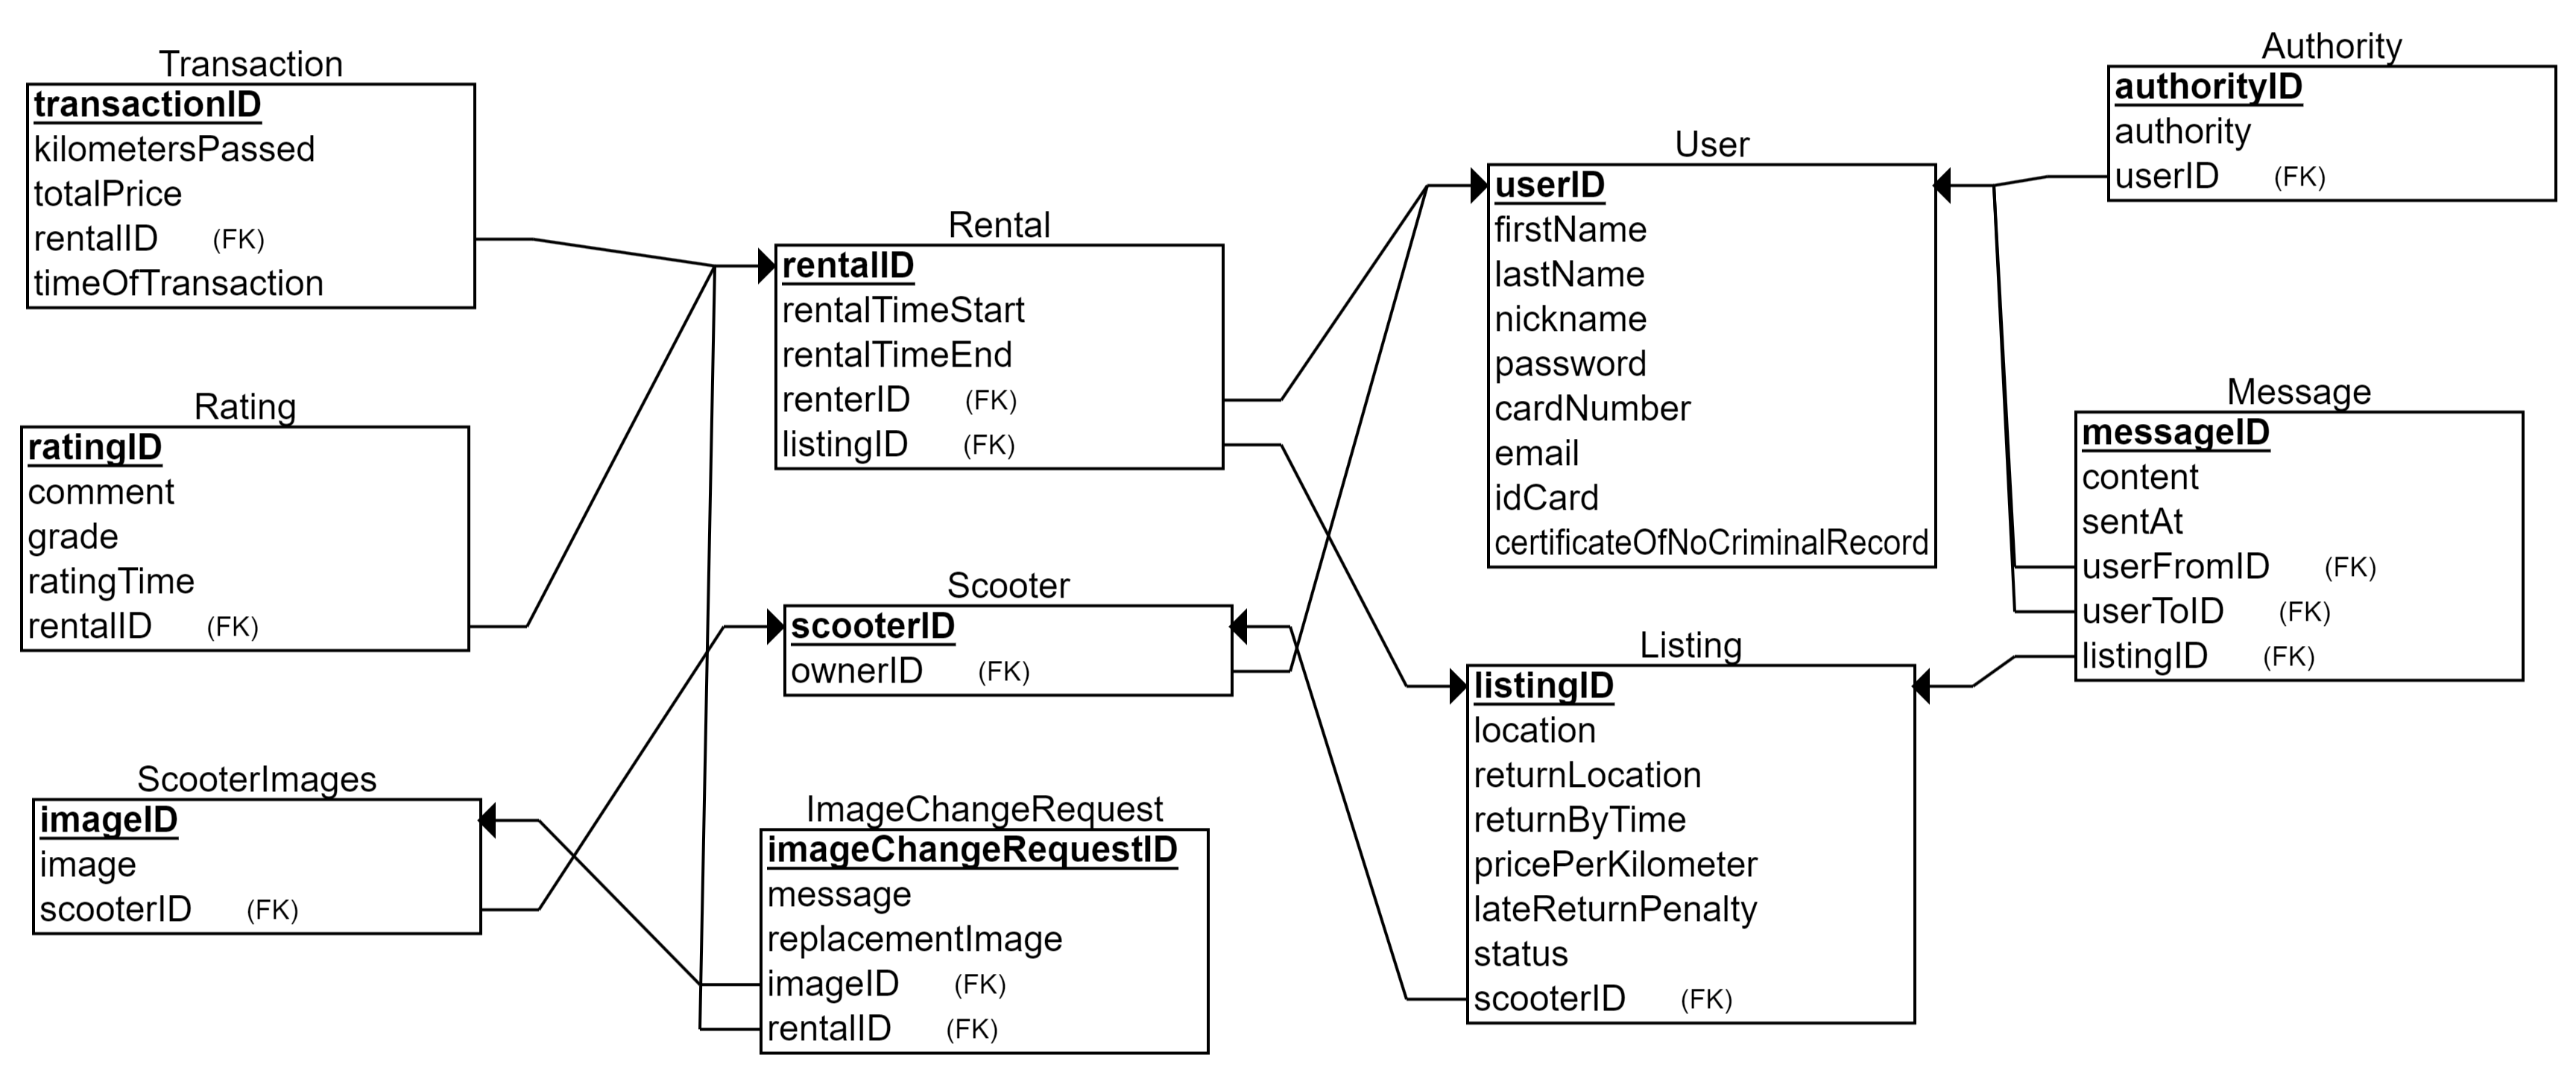
\includegraphics[width=0.8\textwidth]{dijagrami/relacijski_model_baza.png}
					\caption{E-R dijagram baze podataka}
					\label{fig:your_label}
				\end{figure}
			
			\eject
			
			
		\section{Dijagram razreda}
		
			\noindent Dijagrami razreda predstavljaju skup razreda koji su dio backend segmenta MVC arhitekture. Ti razredi nasljeđuju Controller razred. Metode unutar tih razreda manipuliraju s DTO (Data Transfer Object) koji su dohvaćeni kroz implementirane metode u Entitet i Servisi razredima. Kontrolni razredi implementiraju metode koje vraćaju JSON datoteke s odgovarajućim HTML status kodom. \\
			
			\indent Razredi su logički grupirani prema pravima pristupa određenih aktera. Ova organizacija pomaže smanjiti prenapučenost unutar dijagrama, gdje su prikazane samo ovisnosti između razreda koji pripadaju istom segmentu dijagrama. Informacije o nazivima i tipovima atributa unutar razreda omogućuju zaključivanje vrste ovisnosti među različitim razredima. \\
		
			\begin{figure}[H]
				\centering
				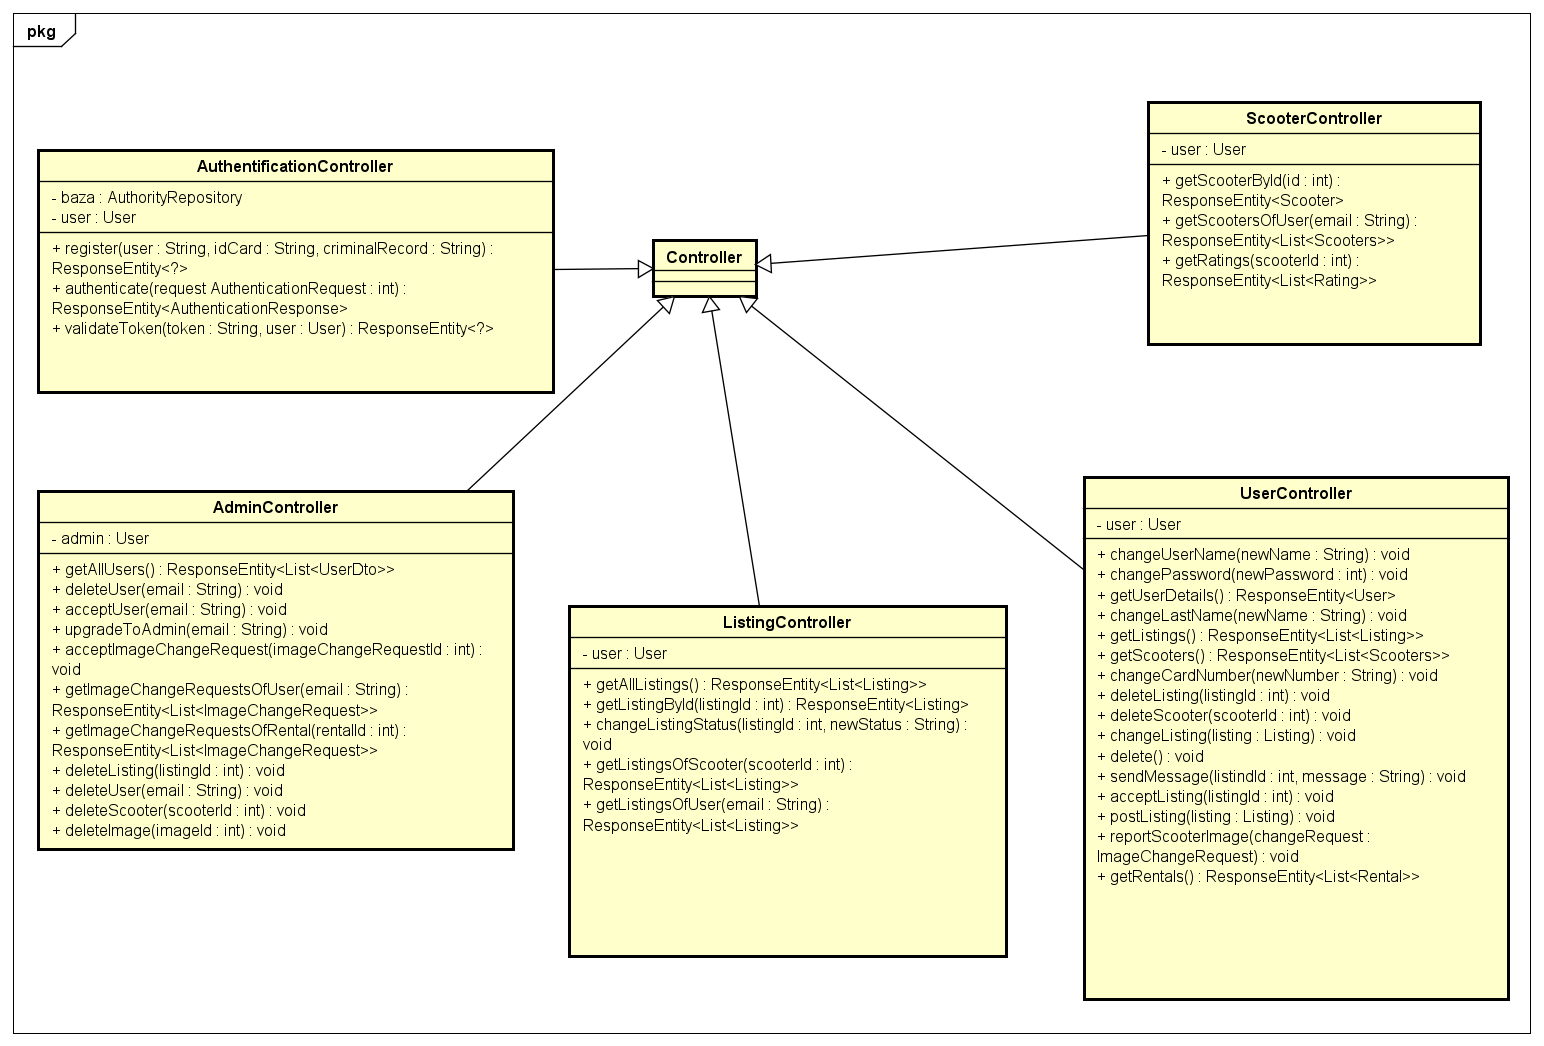
\includegraphics[width=0.8\textwidth]{dijagrami/ControllersDiagram.png}
				\caption{Dijagram razreda - dio Controllers}
				\label{fig:your_label}
			\end{figure}
			
			\begin{figure}[H]
				\centering
				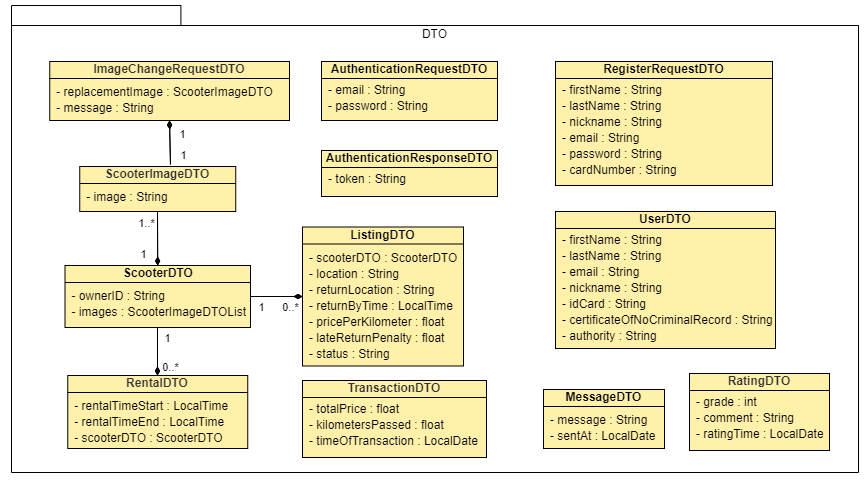
\includegraphics[width=0.8\textwidth]{dijagrami/DTO_dijagram.png}
				\caption{Dijagram razreda - dio Data Transfer Objects}
				\label{fig:your_label}
			\end{figure}
			
			\indent Servisi i Entiteti predstavljaju dvije ključne komponente koji primjenjuju arhitektonski obrazac poznat kao "Service-Oriented Architecture" (SOA) ili "Domain-Driven Design" (DDD). \\
			
			 \indent Entiteti predstavljaju objekte u bazi podataka koji imaju svoj identitet. Svaki entitet ima svoje primarne i sekundarne ključeve kojima su vezani za ostale entitete. \\
			 
			 \indent Servisi predstavljaju komponente sustava koje obavljaju određene operacije ili funkcionalnosti. Oni sadrže poslovnu logiku i nude specifične usluge koje se mogu pozvati iz drugih dijelova sustava. \\
			 
			\begin{figure}[H]
				\centering
				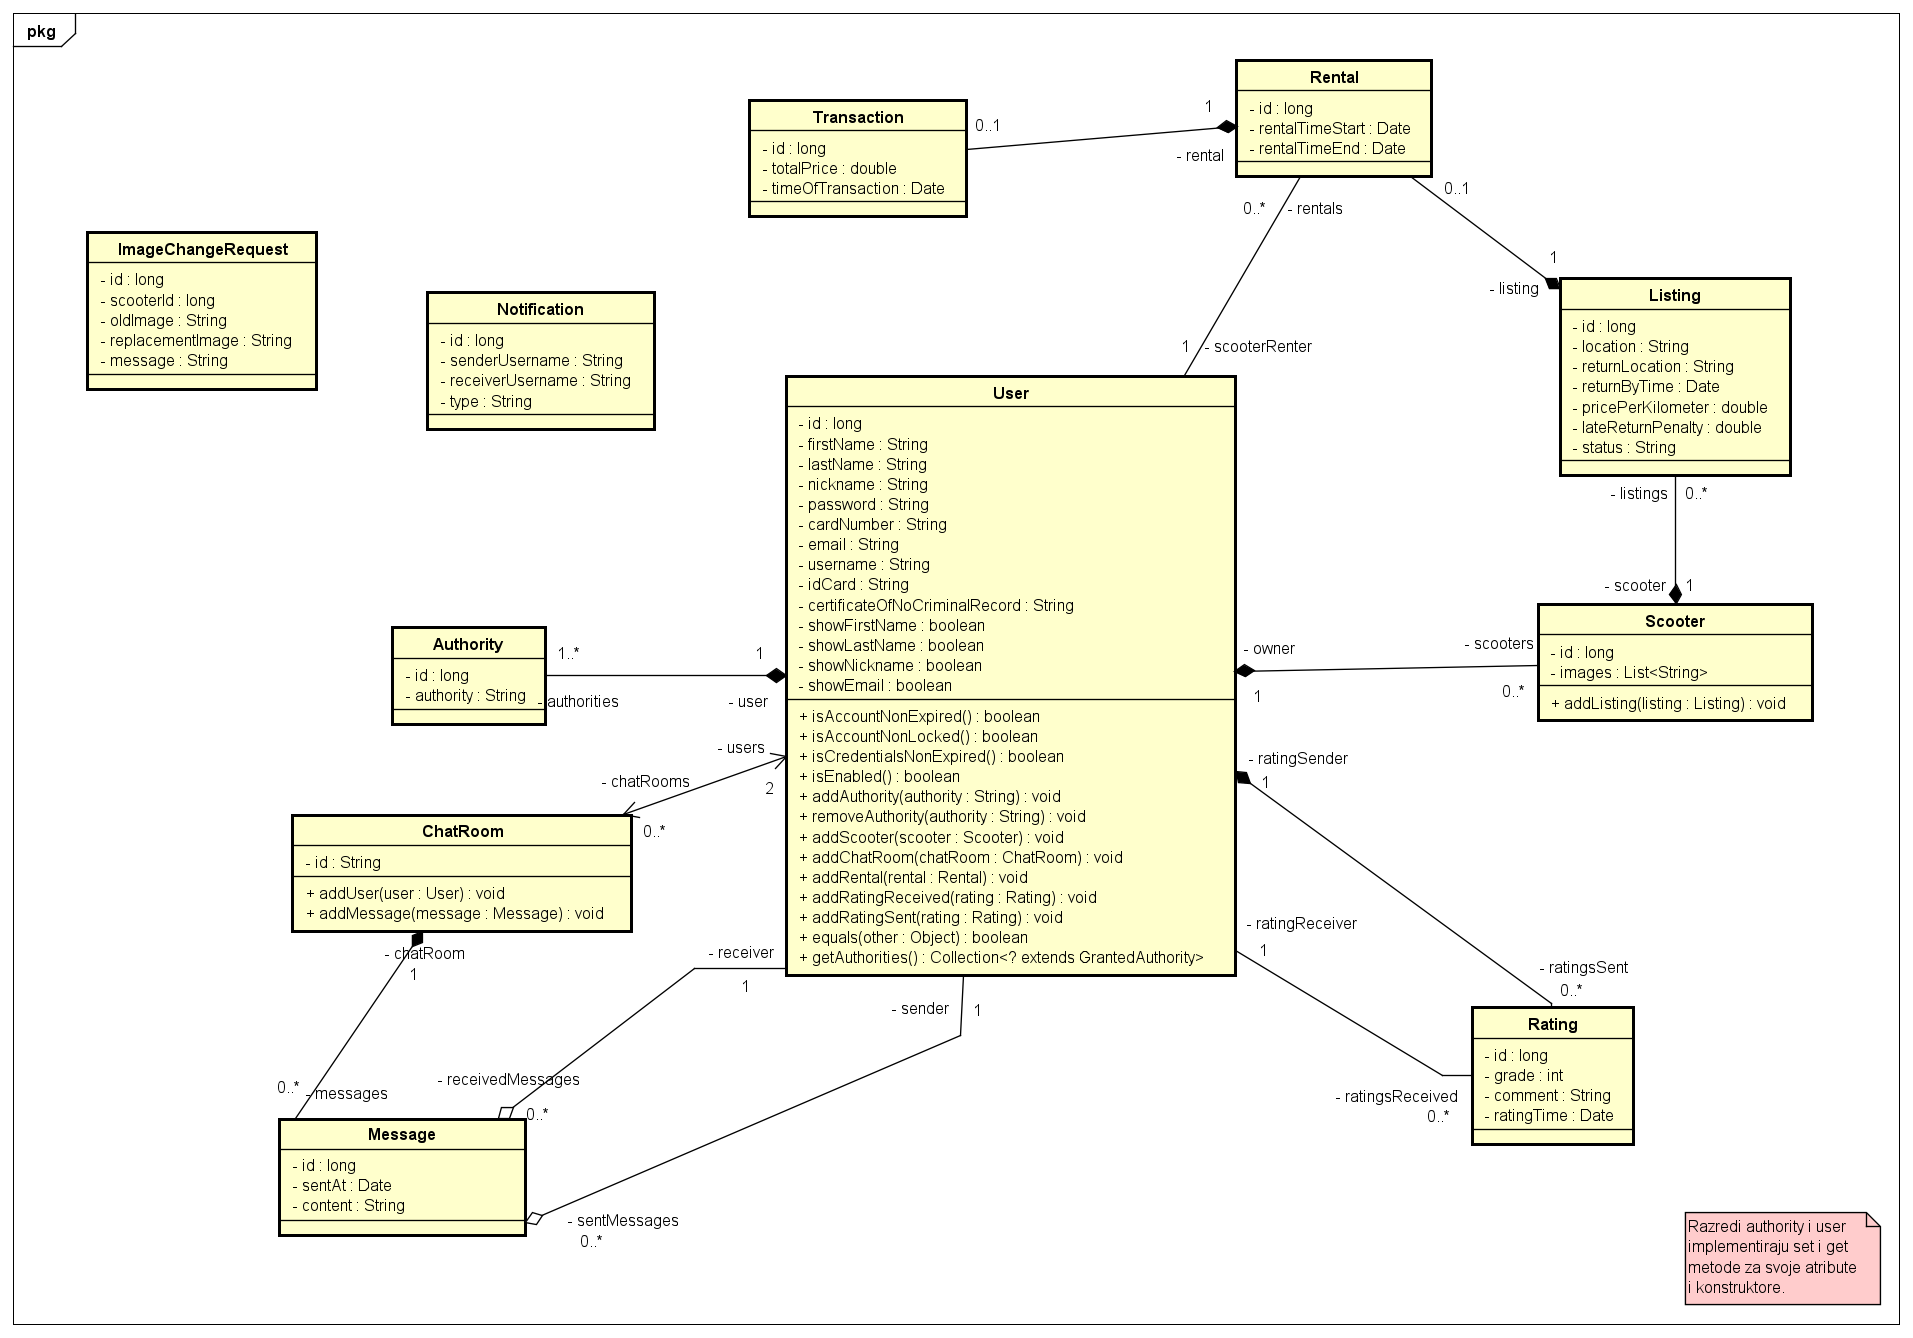
\includegraphics[width=0.8\textwidth]{dijagrami/entiteti.png}
				\caption{Dijagram razreda - dio Entiteti}
				\label{fig:your_label}
			\end{figure}
			
			\begin{figure}[H]
				\centering
				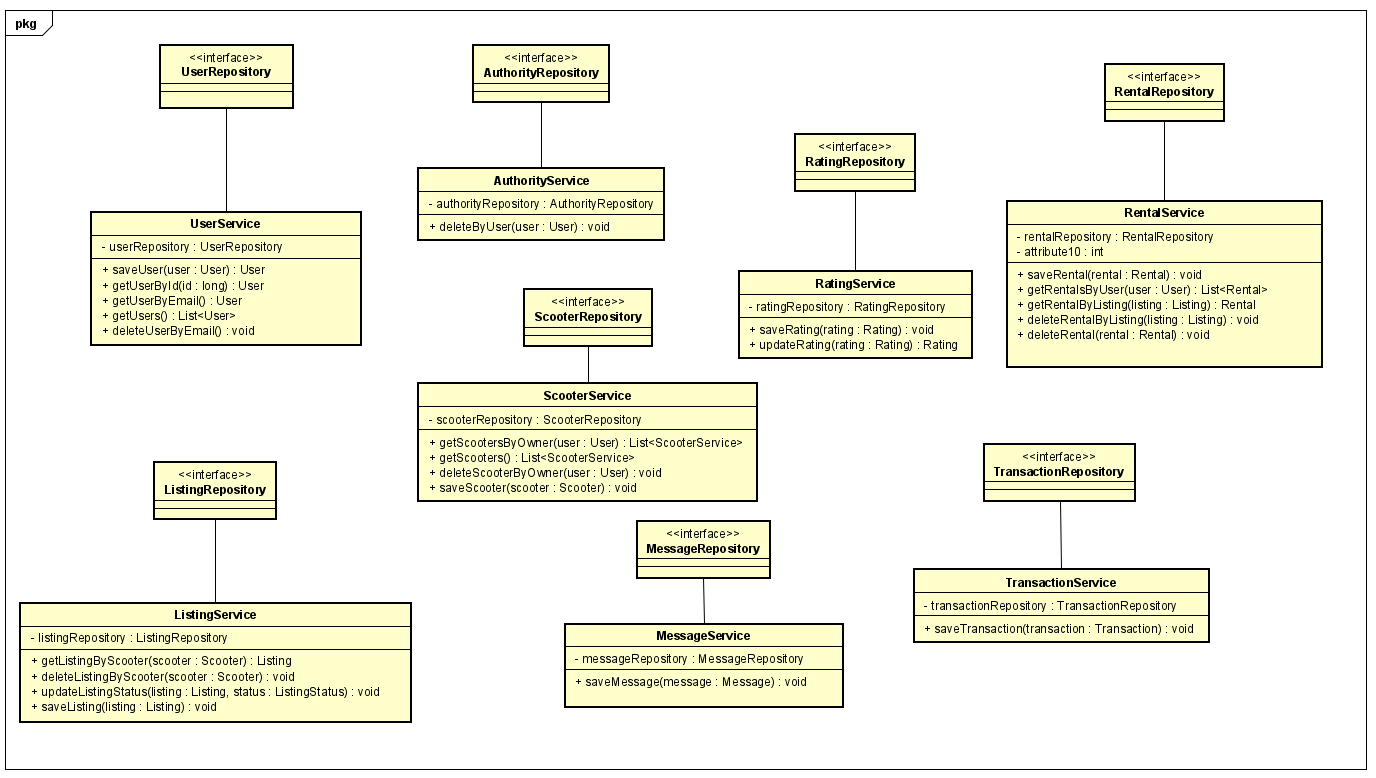
\includegraphics[width=0.8\textwidth]{dijagrami/servisi.png}
				\caption{Dijagram razreda - dio Servisi}
				\label{fig:your_label}
			\end{figure}
			
			
			\eject
		
		\section{Dijagram stanja}
			
			
			\textbf{\textit{dio 2. revizije}}\\
			
			\textit{Potrebno je priložiti dijagram stanja i opisati ga. Dovoljan je jedan dijagram stanja koji prikazuje \textbf{značajan dio funkcionalnosti} sustava. Na primjer, stanja korisničkog sučelja i tijek korištenja neke ključne funkcionalnosti jesu značajan dio sustava, a registracija i prijava nisu. }
			
			
			\eject 
		
		\section{Dijagram aktivnosti}
			
			\indent Dijagram aktivnosti primjenjuje se za modeliranje upravljačkog i podatkovnog toka. Pogodan je za opisivanje sinkronizacije i konkurentnosti. Dijagram aktivnosti ne primjenjuje se za modeliranje događajima poticanog ponašanja. U modeliranju toka upravljanja novi korak se izvršava nakon završenog prethodnog. \\
			
			\indent Dijagram aktivnosti 4.7 prikazuje jednostavan proces iznajmljivanja romobila. 
			Korisnik se prijavljuje, odabire romobil, te nakon kontakta s iznajmljivačem, proces iznajmljivanja postaje aktivan. \\
			
			\begin{figure}[H]
				\centering
				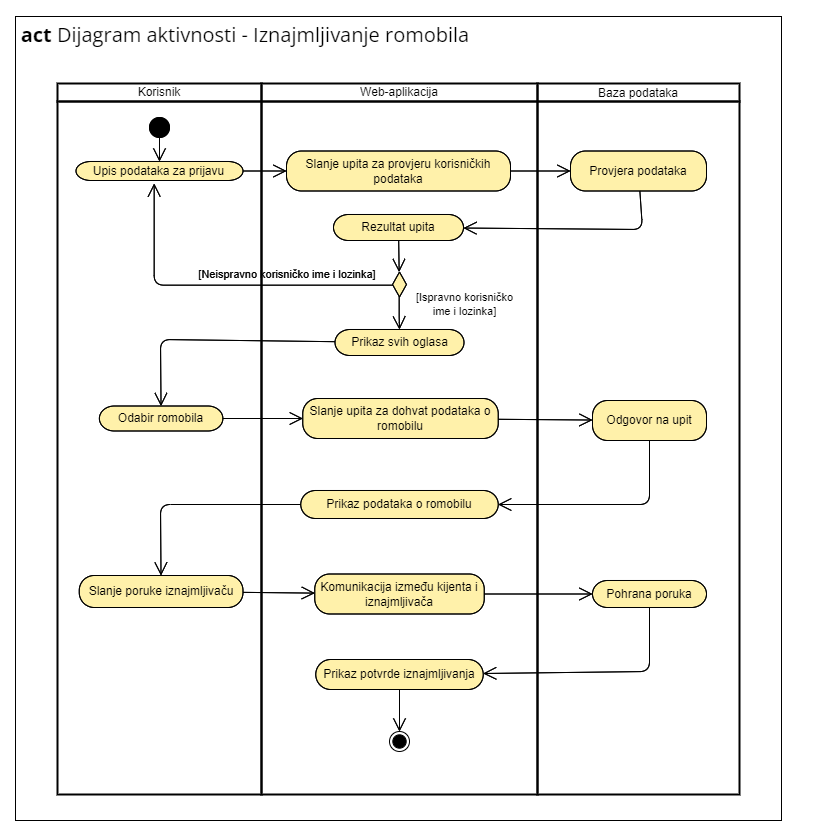
\includegraphics[width=0.8\textwidth]{dijagrami/aktivnost.png}
				\caption{Dijagram aktivnosti}
				\label{fig:your_label}
			\end{figure}
			
			\eject
			
		\section{Dijagram komponenti}
		
			\textbf{\textit{dio 2. revizije}}\\
		
			 \textit{Potrebno je priložiti dijagram komponenti s pripadajućim opisom. Dijagram komponenti treba prikazivati strukturu cijele aplikacije.}